\documentclass{article}

\title{PhD Outline}
\author{Wellen}
\date{\today}

\usepackage[utf8]{inputenc}
\usepackage[margin=1in]{geometry}
\usepackage{url, appendix, pdfpages, subcaption} %for inputting urls, appendices, outside docs, and placing multiple pictures in the same figure
%http://blog.bharatbhole.com/inserting-pages-from-an-external-pdf-document-within-a-latex-document/
\usepackage{float} %[H] tells LaTeX you absolutely want an image there
\usepackage{fancyhdr, enumitem}
\newcommand{\compresslist}{ % Define a command to reduce spacing within itemize/enumerate environments, this is used right after \begin{itemize} or \begin{enumerate}
	\setlength{\itemsep}{0pt}
	\setlength{\parskip}{0pt}
	\setlength{\parsep}{10pt}
}
\usepackage{amsmath, amssymb, mathrsfs, dsfont, amsthm,  cancel}
\usepackage[mathscr]{eucal} %for getting less bold and swirlier math scripts
\usepackage{graphicx, tikz, wrapfig} %for figures, figure creation, and haveing text to the left of a figure
\allowdisplaybreaks[1]

\usepackage{titlesec}
%\titlespacing*{\subsubsection}{0pt}{0\baselineskip}{\baselineskip}

%Places the title information in the header
\makeatletter         
%\def\@maketitle{{\bfseries\@title}\\ \@author \\ \@date }


%%%%%%%%%%%%%%%%%%%%%%%%%%%%%%%%%%%%%%%%%%%%%%%%%%%%%%%%%%%%%%%%%%%%%%
%
%								MACROS
%
%%%%%%%%%%%%%%%%%%%%%%%%%%%%%%%%%%%%%%%%%%%%%%%%%%%%%%%%%%%%%%%%%%%%%%

%                   Brackets and Parenthesis

\newcommand{\<}{\langle}
\renewcommand{\>}{\rangle}
\renewcommand{\(}{\left(}
\renewcommand{\)}{\right)}
\renewcommand{\[}{\left[}
\renewcommand{\]}{\right]}

%                   Math Blackboard Bold Symbols

\newcommand\Cb{\mathds{C}}
\newcommand\Eb{\mathds{E}}
\newcommand\Fb{\mathds{F}}
\newcommand\Gb{\mathds{G}}
\newcommand\Pb{\mathds{P}}
\newcommand\Qb{\mathds{Q}}
\newcommand\Rb{\mathds{R}}
\newcommand\Zb{\mathds{Z}}
\newcommand\Nb{\mathds{N}}
\newcommand\Vb{\mathds{V}}

%                   mathscr symbols

\newcommand\Ac{\mathscr{A}}
\newcommand\Bc{\mathscr{B}}
\newcommand\Cc{\mathscr{C}}
\newcommand\Dc{\mathscr{D}}
\newcommand\Ec{\mathscr{E}}
\newcommand\Fc{\mathscr{F}}
\newcommand\Gc{\mathscr{G}}
\newcommand\Hc{\mathscr{H}}
\newcommand\Lc{\mathscr{L}}
\newcommand\Mc{\mathscr{M}}
\newcommand\Nc{\mathscr{N}}
\newcommand\Oc{\mathscr{O}}
\newcommand\Pc{\mathscr{P}}
\newcommand\Qc{\mathscr{Q}}
\newcommand\Sc{\mathscr{S}}
\newcommand\Kc{\mathscr{K}}
\newcommand\Jc{\mathscr{J}}
\newcommand\Xc{\mathscr{X}}
\newcommand\Yc{\mathscr{Y}}
\newcommand\Zc{\mathscr{Z}}

%                   shortcuts for greek letters

\newcommand\eps{\epsilon}
\newcommand\om{\omega}
\newcommand\Om{\Omega}
\newcommand\sig{\sigma}
\newcommand\Sig{\Sigma}
\newcommand\Lam{\Lambda}
\newcommand\gam{\gamma}
\newcommand\Gam{\Gamma}
\newcommand\lam{\lambda}
\newcommand\del{\delta}
\newcommand\Del{\Delta}
\newcommand\Chi{\mathcal{X}}

%                   Letters with bars

\newcommand\Wb{\overline{W}}
\newcommand\Mb{\overline{M}}
\newcommand\Xb{\overline{X}}
\newcommand\Yb{\overline{Y}}
\newcommand\Sb{\overline{S}}
\newcommand\Pbb{\overline{\Pb}}
\newcommand\Ebb{\overline{\Eb}}
\newcommand\Acb{\bar{\Ac}}
\newcommand\ab{\overline{a}}
\newcommand\bb{\overline{b}}
\newcommand\hb{\overline{h}}
\newcommand\xb{\bar{x}}
\newcommand\yb{\bar{y}}
\newcommand\zb{\bar{z}}
\newcommand\Ab{\bar{\Ac}}
\newcommand\vb{\bar{v}}
\newcommand\ub{\bar{u}}
\newcommand\qb{\bar{q}}
\newcommand\pb{\bar{p}}
%\newcommand\Vb{\bar{V}}
\newcommand\rhob{\bar{\rho}}
\newcommand\IIb{\bar{\II}}
\newcommand\LLb{\bar{\LL}}
\newcommand{\psib}{\bar{\psi}}
\newcommand{\etab}{\bar{\eta}}
\newcommand{\xib}{\bar{\xi}}

%                   Letters with underlines

\newcommand\Wu{\underline{W}}
\newcommand\Xu{\underline{X}}
\newcommand\Mu{\underline{M}}

%                   Vectors (bolded)

\newcommand\Av{\mathbf{A}}
\newcommand\Fv{\mathbf{F}}
\newcommand\xv{\mathbf{x}}
\newcommand\bv{\mathbf{b}}
\newcommand\pv{\mathbf{p}}
\newcommand\qv{\mathbf{q}}
\newcommand\ev{\mathbf{e}}
\newcommand\yv{\mathbf{y}}
\newcommand\zv{\mathbf{z}}
\newcommand\Yv{\mathbf{Y}}
\newcommand\Hv{\mathbf{H}}
\newcommand\Cv{\mathbf{C}}
\newcommand\mv{\mathbf{m}}
\newcommand\etav{\boldsymbol\eta}
\newcommand\piv{\boldsymbol \pi}
\newcommand\muv{\boldsymbol \mu}
\newcommand\Sv{\textbf S}
\newcommand\Qv{\textbf Q}
\newcommand\zev{\textbf 0}

%                   Letters with Hats

\newcommand\Pbh{\widehat{\Pb}}
\newcommand\Ebh{\widehat{\Eb}}
\newcommand\Qh{\widehat{Q}}
\newcommand\Ih{\widehat{I}}
\newcommand\pih{\widehat{\pi}}
\newcommand\Pih{\widehat{\Pi}}
\newcommand\varphih{\widehat{\varphi}}
\newcommand\Wh{\widehat{W}}
\newcommand\Fh{\widehat{F}}
\newcommand\Yh{\widehat{Y}}
\newcommand\Ah{\widehat{\Ac}}
\newcommand\uh{\widehat{u}}
\newcommand\Uh{\widehat{U}}
\newcommand\vh{\widehat{v}}
\newcommand\fh{\widehat{f}}
\newcommand\Hh{\widehat{H}}
\newcommand\hh{\widehat{h}}
\newcommand\Bh{\widehat{B}}
\newcommand\etah{\widehat{\eta}}
\newcommand\Lh{\widehat{L}}

%                   Letters with Tildes

\newcommand\Ebt{\widetilde{\Eb}}
\newcommand\Pbt{\widetilde{\Pb}}
\newcommand\Act{\widetilde{\Ac}}
\newcommand\Lct{\widetilde{\Lc}}
\newcommand\Gct{\widetilde{\Gc}}
\newcommand\Xct{\widetilde{\Xc}}
\newcommand\Yct{\widetilde{\Yc}}
\newcommand\Zct{\widetilde{\Zc}}
\newcommand\Mt{\widetilde{M}}
\newcommand\Wt{\widetilde{W}}
\newcommand\Bt{\widetilde{B}}
\newcommand\Nt{\widetilde{N}}
\newcommand\Xt{\widetilde{X}}
\newcommand\xt{\widetilde{x}}
\newcommand\ut{\widetilde{u}}
\newcommand\kappat{\widetilde{\kappa}}
\newcommand\at{\widetilde{a}}
\newcommand\Gamt{\widetilde{\Gam}}
\newcommand\Pct{\widetilde{\Pc}}


%         Theorem environments

\newtheoremstyle{mine}% name of the style to be used
  { }% measure of space to leave above the theorem. E.g.: 3pt
  { }% measure of space to leave below the theorem. E.g.: 3pt
  { }% name of font to use in the body of the theorem
  { }% measure of space to indent
  { }% name of head font
  { }% punctuation between head and body
  { }% space after theorem head; " " = normal interword space
  {\thmname{\textbf{#1}}\thmnumber{\textbf{ #2}}:\thmnote{ #3}\\}% Manually specify head

\theoremstyle{mine}
\newtheorem{thm}{Theorem}[section]
\newtheorem{cor}[thm]{Corollary}
\newtheorem{prop}[thm]{Proposition}
\newtheorem{defn}[thm]{Definition}
\newtheorem{rmk}[thm]{Remark}
\newtheorem{lem}[thm]{Lemma}
\newtheorem{assumption}[thm]{Assumption}


%                   other macros

\newcommand{\dd}{\partial}
\newcommand{\ind}{\perp \! \! \! \perp}
\newcommand\ii{\mathtt{i}}
\renewcommand\d{\mathrm{d}}
\newcommand\ee{\mathrm{e}}
\newcommand\BS{\textrm{BS}}
\newcommand\ko{\mathrm{ko}}
\newcommand\ki{\mathrm{ki}}
\newcommand\rb{\mathrm{rb}}
\newcommand\eu{\mathrm{eu}}

%          other


\newcommand\Ib{\mathds{1}}
\renewcommand\Re{\operatorname{Re}}
\renewcommand\Im{\operatorname{Im}}
\newcommand{\nuba}[1]{\overline{\nu_{#1}^\ast}}
\newcommand{\tab}{\hspace{.4 in}}
\newcommand{\enter}{\vspace{.15 in}}
\newcommand{\fa}{\forall}
\newcommand{\tf}{\therefore}
\newcommand{\indep}{\raisebox{0.05em}{\rotatebox[origin=c]{90}{$\models$}}}
\newcommand{\nth}[2]{#1^{\text{\tiny #2}}}
\newcommand{\xRightarrow}[2][]{\ext@arrow 0359\Rightarrowfill@{#1}{#2}}
\newcommand{\myeq}[1]{\mathrel{\overset{\makebox[0pt]{\mbox{\small {#1}}}}{=}}}
\newcommand{\since}{\reflectbox{\rotatebox[origin=c]{180}{$\therefore$}}}
\makeatother


\begin{document}

\title

\section{Generic Model from Literature}

	A Simple Dynamical System - \underline{Economic Dynamics: Phase Diagrams and Their Economic Application} by Ronald Shone
	
	\begin{align}
		q_d =& a - bp && b > 0 \label{eq:qd1}\\ 
		q_s =& c + fp && f > 0 \label{eq:qs1}\\ 
		\frac{\d p}{\d t} =& \alpha(q_d - q_s) = \alpha(b+f)p - \alpha(a-c) && \alpha > 0 \label{eq:pt1}
	\end{align}
	There is an equilibrium at $p(t) = \frac{a-c}{b+f} + \[p_0 - \(\frac{a-c}{b+f}\)\]e^{-\alpha(b+f)t}$
	%p(0) = p_0
	$q_d,\ q_s,\ \&\ p$ are continuous functions of time.
	
	Analyzing the Jacobian of this system for $q_d$ and $p$ we get
	$$\begin{matrix}
		0 & -b\\
		0 & \alpha(b+f)
	\end{matrix}.$$
	From here I calculated the eigenvalues to find $\lambda_1 = \alpha(b+f)$ and $\lambda_2 = 0$. $\lambda_2 = 0$ could be a problem if we were dealing with a nonlinear system, however this is a linear system so the behavior of the fixed points is determined by $\lambda_1$. This means that if $\lambda_1 < 0 $ the system is stable, and if $\lambda_1 > 0$ then it is unstable. However we know that $\lambda_1 > 0 $, since the restraints on our system require that $\alpha>0$, $b>0$, and $f>0$. For $b$ and $f$, this is to account for how we know demand decreases and supply increases as price increases, which are well established results in economics except in extreme outliers. $\alpha >0$ comes from examining $(q_d - q_s)$. If $\alpha < 0$, then we could rewrite it as $|\alpha|(q_s - q_d)$, but demand does not shift to meet supply, supply and price both shift to meet demand in an economy. Thus we see that for all possible versions of this system, we have an unstable equilibrium.  
	
	\begin{figure}[h]
		\centering
			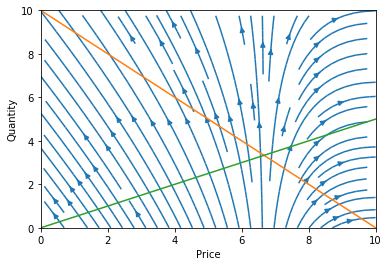
\includegraphics[width = 0.6\columnwidth]{Figures/simple_system.png}
		\caption{The vector field plot of the system described in \eqref{eq:qd1}}
		\label{fig:model1} 
	\end{figure}

Numerically I analyzed the system with $a = 10,\ b = 1,\ c = 0,\ f = 0.5,$ and $alpha = 0.5$. The orange line is the quantity demanded that I assumed in equation \eqref{eq:qd1}. The green line is the quantity supplied that I assumed in equation \eqref{eq:qs1}. Consumer utility for the product is assumed to not change over time, and so these demand lines are both held constant over time. We see in Figure \ref{fig:model1} the equilibrium point of $(6 \frac{2}{3}, 3 \frac{1}{3})$ in the classic supply and demand system, and also how for this system a price of $6 \frac{2}{3}$ does not change. Further, the quantity demanded can also be thought of as the maximum quantity sold at any given price, so only the dynamics in the bottom left half of the plot should be analyzed.

As expected from the analysis, in figure \ref{fig:model1} we see that prices do not flow towards the price equilibrium, but instead to move away from it. This is made even more clear in figure \ref{fig:model1_time_price}, which is the time evolution of price. In this system we see that the price can only reach the equilibrium of $6 \frac{2}{3}$ by already starting at that value. This is in direct conflict to current theory which states that prices will converge to equilibrium. To achieve a dynamical system that fits a stable equilibrium, we must break one of our main underlying economic assumptions.

For this model the dynamics don't make sense. Also, this model does not indicate at all how things evolve if the demand or supply shifts. With the underlying issues in the model, it is not clear that any conclusions drawn would be meaningful. There is plenty to explore in this field.

	\begin{figure}
		\centering
			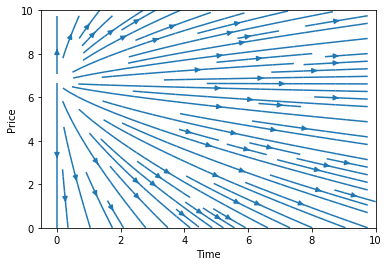
\includegraphics[width = 0.6\columnwidth]{Figures/simple_priceOverTime.png}
		\caption{The evolution of price over time according to \eqref{eq:pt1}}
		\label{fig:model1_time_price} 
	\end{figure}



%%%%%%%%%%%%%%%%%%%%%%%%%%%%%%%%%%%%%%%%%%%%%%%%%%%%%%%%%%%%%%%%%%%%%%%%%%%%%%%%%%%%%%%%%%%%%%%%%%%%%%%%%%%%%%%%%%%%%%%%%%%%%%%%%%%%%%%%
%%%%%%%%%%%%%%%%%%%%%%%%%%%%%%%%%%%%%%%%%%%%%%%%%%%%%%%%%%%%%%%%%%%%%%%%%%%%%%%%%%%%%%%%%%%%%%%%%%%%%%%%%%%%%%%%%%%%%%%%%%%%%%%%%%%%%%%%

\section{My Model}

Here I am exploring different concepts that I think belong in a model of supply and demand.

I am working with at least five different curves:
\begin{enumerate}
	\item The supply curve: a plot of the quantity willing to be supplied for any given price. This may change over time. Note that this is quantity vs. price.
	\item The demand curve: a plot of the quantity that consumers are willing and able to purchase for any given price. This may change over time. Note that this is quantity vs. price.
	\item Demand over time: the quantity of goods actually purchased from a marketplace at time $t$. Note that this is quantity vs. time.
	\item Supply over time: the amount of goods contributed to the marketplace at time $t$. Note that this is quantity vs. time.
	\item Price over time: how prices that the good(s) are sold at change over time. Note that this is price vs. time. Marketplace Equilibrium is defined as the price where the quantity purchased at time $t$ is equivalent to the quantity supplied at time $t$. Marketplace equilibrium should theoretically also be an equilibrium of the dynamical system. 
\end{enumerate}
This list 

\subsection{The Evolution of Supply Over Time}
\begin{itemize}
	\item Quantity supplied and quantity demanded are positively correlated
	\item Changes in the ``supply curve'' and ``demand curve'' ought to change over time
	\item My model should be able to handle non-linear supply and demand curves. 
	\begin{itemize}
		\item Start with quadratic case, this is often used to describe global supply and demand
	\end{itemize}
\end{itemize}

\subsubsection{Constant Shifts in the Curves}
The quantity supplied and quantity demanded are positively correlated. As demand increases supply increases to match, but by a smaller amount. This smaller amount allows the price to also increase, creating greater profit margins. This is in an idealized market of course, since if there are competitors, that could keep a company from raising their prices. However, a company will never purposefully supply more than the amount demanded since that will drive down prices and profit margin, while also increasing stocks keeping profit down in the future. When demand quantity decreases we would then expect the supply quantity to decrease more than this. The reasoning is similar to why it would increase less than with demand increase. We can call this amount of disconnect in change $\delta$. $\delta$ is then approximately $(\frac{dS}{dq} - \frac{dD}{dq})^{-1}$ according to the linear supply and demand model taught in macroeconomics textbooks.

Thus we have that 
\begin{align}
	\dot{q}_S(t) = (\frac{dS}{dq} - \frac{dD}{dq})^{-1}(\dot{q}_D(t)) \label{eq:dqs_1}\\
	& \ \ \ +\eps\ddot{q}_D(t)  \label{eq:predict_demand}
\end{align}
From equation \eqref{eq:dqs_1} we come to the big question of what does $\frac{dS}{dq}$ and $\frac{dD}{dq}$ mean? These are the slopes of the linear lines in the model displayed in Figure \ref{fig:SnD}. As written, this model only allows for the shifts in intercepts as shown in Figure \ref{fig:SnD}. Only shifts are allowed because we do not allow the slopes to vary over time, and the way this is written assumes that we are working with linear underlying functions.   

\begin{figure}
	\centering
		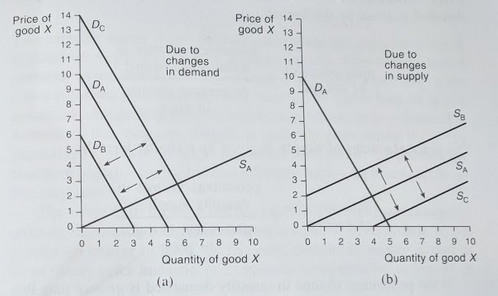
\includegraphics[width = 0.6\columnwidth]{Figures/SnD.png}
	\caption{Supply and Demand as a classic linear system.}
	\label{fig:SnD} 
\end{figure}

Even though it is linear, another aspect to the model is that firms may attempt to predict the necessary supply in the future. This is included as a second derivative term in \eqref{eq:predict_demand}.
It would be optimizing in that if they expect things to change quickly, they can try not to run out of stock in stores. This may be especially relevant for the case of perishable goods where rather than always being behind demand until it reaches a equilibrium, companies are trying to be ahead and always have supplied what the consumers will purchase. This would likely need an unknown constant in front of the term that is less than one (it should have less cost associated to under-perform in this term). 




\subsubsection{Non-linear shifts}
The model in \ref{eq:dqs_1} is still missing the dependence on time. Once we allow a time dependence in $\frac{dS}{dq}$ and $\frac{dD}{dq}$. Even if we do that though, I have still only thought about them as linear so that we can calculate a constant coefficient out front of $(q_D +\dot{q}_D)$. What happens if the slope is non-linear so that it matters what the current market quantity/prices are?

\begin{align}
	\dot{q}_S(t) = & \left[(\frac{dS}{dq} - \frac{dD}{dq})(t)\right]^{-1}(q_D(t) +\dot{q}_D(t)) +\eps\ddot{q}_D(t) \label{eq:dqs_2}
\end{align}

\subsubsection{Quadratic Underlying Curve}

%%%%%%%%%%%%%%%%%%%%%%%%%%%%%%%%%%%%%%%%%%%%%%%%%%%%%%%%%%%%%%%%%%%%%%%%%%%%%%%%%%%%%%%%%%%%%%%%%%%%%%%%%%%%%%%%%%%%%%%%%%%%%%%%%%%%%%%%

\subsection{The Evolution of Quantity Demanded}
We also want to look into how the quantity demanded changes changes over time. I believe as a consumer, that this will be based mostly on the price, where $p$ is the transaction price taking place in the market. There is also something to be said for ease of access and rarity of the goods, so I believe that a positive quadratic term makes sense for the supply available effecting the quantity demanded. I argue that change in quantity supplied is not noticeable to a consumer. Either the store has the good or it does not, I have no idea what others are up to. Thus the change in quantity supplied term is left out. 

Something interesting that I always thought was left out is rarity. It is really obvious in trading cards, but also in Grey Poupon mustard. Something can be more expensive and that attracts people to it perhaps because of ideas of luxury. Because of this sort of thing, I do not believe that the interaction between supply and demand is linear, so then the question is what kind of non-linearity makes sense. 

\begin{equation}
		\dot{q}_D = - c_1 \dot{p} - c_2(q_S-c_3)^3
\end{equation}

In this system we can assume that companies may change their supply without a large effect on consumption, as long as the consumers can still easily access a good (or highly value the rarity of it which is handled in $c_3$).


%%%%%%%%%%%%%%%%%%%%%%%%%%%%%%%%%%%%%%%%%%%%%%%%%%%%%%%%%%%%%%%%%%%%%%%%%%%%%%%%%%%%%%%%%%%%%%%%%%%%%%%%%%%%%%%%%%%%%%%%%%%%%%%%%%%%%%%%

\section{Taking Stocks of Goods into Account}
The stock of excess supplied goods also needs to be taken into account. This is only relevant for the case of non-perishable goods, just as I would guess that the second derivative term is only relevant for the case of perishable goods. Do companies want at least a certain amount stockpiled? The only difference in the model is that companies would make less money, so we can ignore this in terms of understanding the dynamics. One major difference is that the as stockpiles grow, prices tend to drop as a way of clearing them out. So it's not just about the amount supplied, but the amount in total available that determines changes in price. We definitely know that 
\begin{equation*}
	\dot{b} = q_s - q_d
\end{equation*}



%%%%%%%%%%%%%%%%%%%%%%%%%%%%%%%%%%%%%%%%%%%%%%%%%%%%%%%%%%%%%%%%%%%%%%%%%%%%%%%%%%%%%%%%%%%%%%%%%%%%%%%%%%%%%%%%%%%%%%%%%%%%%%%%%%%%%%%%
%%%%%%%%%%%%%%%%%%%%%%%%%%%%%%%%%%%%%%%%%%%%%%%%%%%%%%%%%%%%%%%%%%%%%%%%%%%%%%%%%%%%%%%%%%%%%%%%%%%%%%%%%%%%%%%%%%%%%%%%%%%%%%%%%%%%%%%%

\section{Problems}
\begin{itemize}
	\item It seems like it would be less relevant/useful to model the surplus quantity supplied, than changes in the quantity demanded and the quantity supplied. This is partially because then when we see changes (since presumable preferences do have the possibility of changing over time) we can relate this to the model better.
	\item I don't think S and D should be rates but functions that are greater than or equal to 0. This way aggregate supply and aggregate demand could also be modeled in the same system, and these are generally not considered to be linear.
\end{itemize}


\end{document}